\documentclass[man,floatsintext]{apa6}
\usepackage{lmodern}
\usepackage{amssymb,amsmath}
\usepackage{ifxetex,ifluatex}
\usepackage{fixltx2e} % provides \textsubscript
\ifnum 0\ifxetex 1\fi\ifluatex 1\fi=0 % if pdftex
  \usepackage[T1]{fontenc}
  \usepackage[utf8]{inputenc}
\else % if luatex or xelatex
  \ifxetex
    \usepackage{mathspec}
  \else
    \usepackage{fontspec}
  \fi
  \defaultfontfeatures{Ligatures=TeX,Scale=MatchLowercase}
\fi
% use upquote if available, for straight quotes in verbatim environments
\IfFileExists{upquote.sty}{\usepackage{upquote}}{}
% use microtype if available
\IfFileExists{microtype.sty}{%
\usepackage{microtype}
\UseMicrotypeSet[protrusion]{basicmath} % disable protrusion for tt fonts
}{}
\usepackage{hyperref}
\hypersetup{unicode=true,
            pdftitle={Selective sampling and inductive inference: Drawing inferences based on observed and missing evidence},
            pdfauthor={Brett Hayes, Stephanie Banner, Suzy Forrester, \& Danielle J. Navarro},
            pdfkeywords={Inductive reasoning; property inference},
            pdfborder={0 0 0},
            breaklinks=true}
\urlstyle{same}  % don't use monospace font for urls
\usepackage{graphicx,grffile}
\makeatletter
\def\maxwidth{\ifdim\Gin@nat@width>\linewidth\linewidth\else\Gin@nat@width\fi}
\def\maxheight{\ifdim\Gin@nat@height>\textheight\textheight\else\Gin@nat@height\fi}
\makeatother
% Scale images if necessary, so that they will not overflow the page
% margins by default, and it is still possible to overwrite the defaults
% using explicit options in \includegraphics[width, height, ...]{}
\setkeys{Gin}{width=\maxwidth,height=\maxheight,keepaspectratio}
\IfFileExists{parskip.sty}{%
\usepackage{parskip}
}{% else
\setlength{\parindent}{0pt}
\setlength{\parskip}{6pt plus 2pt minus 1pt}
}
\setlength{\emergencystretch}{3em}  % prevent overfull lines
\providecommand{\tightlist}{%
  \setlength{\itemsep}{0pt}\setlength{\parskip}{0pt}}
\setcounter{secnumdepth}{0}
% Redefines (sub)paragraphs to behave more like sections
\ifx\paragraph\undefined\else
\let\oldparagraph\paragraph
\renewcommand{\paragraph}[1]{\oldparagraph{#1}\mbox{}}
\fi
\ifx\subparagraph\undefined\else
\let\oldsubparagraph\subparagraph
\renewcommand{\subparagraph}[1]{\oldsubparagraph{#1}\mbox{}}
\fi

%%% Use protect on footnotes to avoid problems with footnotes in titles
\let\rmarkdownfootnote\footnote%
\def\footnote{\protect\rmarkdownfootnote}


  \title{Selective sampling and inductive inference: Drawing inferences based on observed and missing evidence}
    \author{Brett Hayes\textsuperscript{1}, Stephanie Banner\textsuperscript{1}, Suzy Forrester\textsuperscript{1}, \& Danielle J. Navarro\textsuperscript{1}}
    \date{}
  
\shorttitle{xxx}
\affiliation{
\vspace{0.5cm}
\textsuperscript{1} University of New South Wales, Australia}
\keywords{Inductive reasoning; property inference\newline\indent Word count: X}
\usepackage{csquotes}
\usepackage{upgreek}
\captionsetup{font=singlespacing,justification=justified}

\usepackage{longtable}
\usepackage{lscape}
\usepackage{multirow}
\usepackage{tabularx}
\usepackage[flushleft]{threeparttable}
\usepackage{threeparttablex}

\newenvironment{lltable}{\begin{landscape}\begin{center}\begin{ThreePartTable}}{\end{ThreePartTable}\end{center}\end{landscape}}

\makeatletter
\newcommand\LastLTentrywidth{1em}
\newlength\longtablewidth
\setlength{\longtablewidth}{1in}
\newcommand{\getlongtablewidth}{\begingroup \ifcsname LT@\roman{LT@tables}\endcsname \global\longtablewidth=0pt \renewcommand{\LT@entry}[2]{\global\advance\longtablewidth by ##2\relax\gdef\LastLTentrywidth{##2}}\@nameuse{LT@\roman{LT@tables}} \fi \endgroup}


\usepackage{lineno}

\linenumbers

\authornote{Add complete departmental affiliations for each author here. Each new line herein must be indented, like this line.

Enter author note here.

Correspondence concerning this article should be addressed to Brett Hayes, School of Psychology, University of New South Wales, NSW 2052, Australia. E-mail: \href{mailto:B.Hayes@unsw.edu.au}{\nolinkurl{B.Hayes@unsw.edu.au}}}

\abstract{
We propose and test a Bayesian model of property induction with evidence that has been selectively sampled leading to ``censoring'' or exclusion of potentially relevant data.


}

\begin{document}
\maketitle

Xu and Tenenbaum (2007) wrote an earlier paper on sampling.

\hypertarget{methods}{%
\section{Methods}\label{methods}}

We report how we determined our sample size, all data exclusions (if any), all manipulations, and all measures in the study.

\hypertarget{participants}{%
\subsection{Participants}\label{participants}}

There were 114 participants in the category sampling condition and 111 in the property sampling condition.

\hypertarget{material}{%
\subsection{Material}\label{material}}

\hypertarget{procedure}{%
\subsection{Procedure}\label{procedure}}

\hypertarget{data-analysis}{%
\subsection{Data analysis}\label{data-analysis}}

\hypertarget{results}{%
\section{Results}\label{results}}

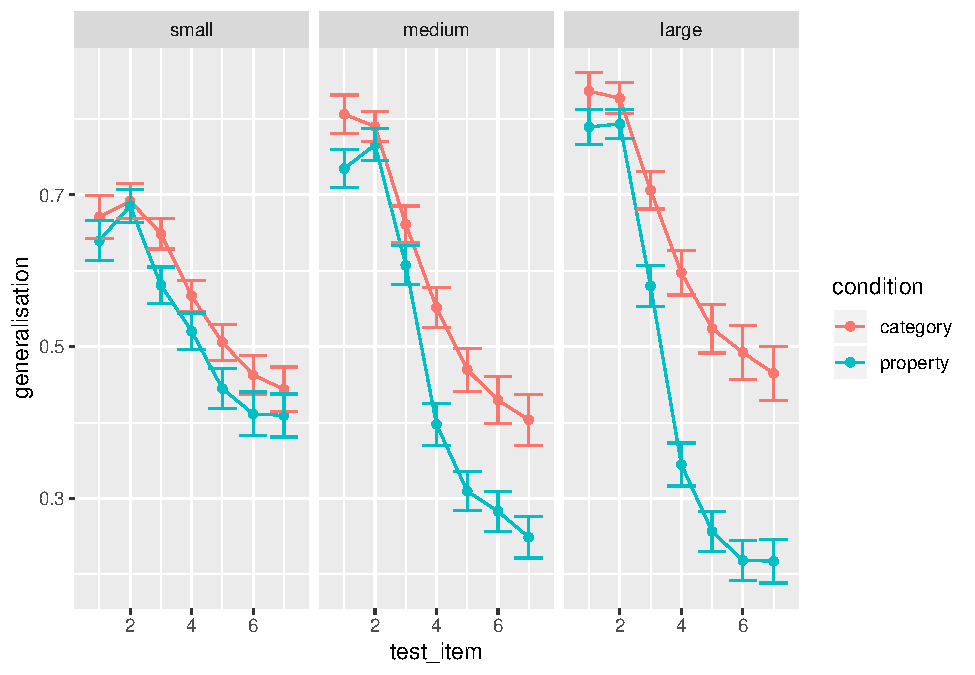
\includegraphics{samplingframes_files/figure-latex/samplesize_plot-1.pdf}

\begin{table}[tbp]
\begin{center}
\begin{threeparttable}
\caption{\label{tab:regression}Regression table for a model with fixed effects only.}
\begin{tabular}{lllll}
\toprule
Predictor & \multicolumn{1}{c}{$b$} & \multicolumn{1}{c}{95\% CI} & \multicolumn{1}{c}{$t(4721)$} & \multicolumn{1}{c}{$p$}\\
\midrule
Intercept & 1.77 & $[1.65$, $1.90]$ & 28.92 & < .001\\
Conditionproperty & -0.50 & $[-0.58$, $-0.43]$ & -13.26 & < .001\\
Test item & -0.33 & $[-0.35$, $-0.31]$ & -32.07 & < .001\\
N obs & 0.00 & $[-0.01$, $0.01]$ & -0.50 & .619\\
\bottomrule
\end{tabular}
\end{threeparttable}
\end{center}
\end{table}

\hypertarget{discussion}{%
\section{Discussion}\label{discussion}}

\newpage

\hypertarget{references}{%
\section{References}\label{references}}

\begingroup
\setlength{\parindent}{-0.5in}
\setlength{\leftskip}{0.5in}

\hypertarget{refs}{}
\leavevmode\hypertarget{ref-xut07a}{}%
Xu, F., \& Tenenbaum, J. B. (2007). Sensitivity to sampling in Bayesian word learning. \emph{Developmental Science}, \emph{10}, 288--297.

\endgroup


\end{document}
